% auto-generated by 09_meeting01_energy_breakeven.py -- do not edit
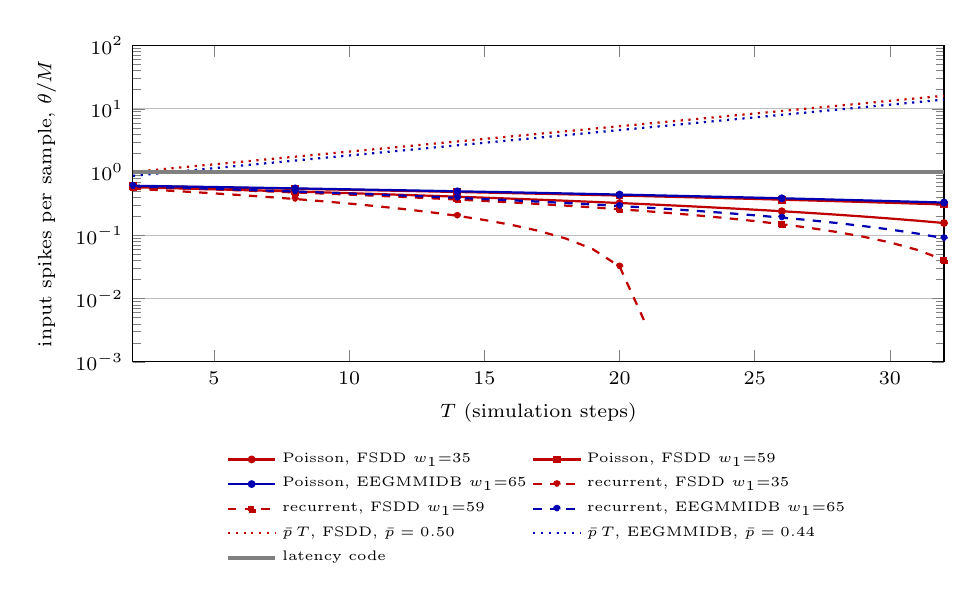
\begin{tikzpicture}[font=\scriptsize]
\begin{axis}[width=0.98\columnwidth, height=5.6cm, xmin=2, xmax=32, ymode=log, ymin=0.001, ymax=100,
  xlabel={$T$ (simulation steps)}, ylabel={input spikes per sample, $\theta/M$},
  legend style={font=\tiny, at={(0.5,-0.25)}, anchor=north, draw=none}, legend columns=2, legend cell align=left, ymajorgrids, yminorgrids=false]
\addplot[solid, thick, color=red!75!black, mark=*, mark size=1pt, mark repeat=6] coordinates {(2,0.5765) (3,0.5625) (4,0.5485) (5,0.5345) (6,0.5205) (7,0.5065) (8,0.4926) (9,0.4786) (10,0.4646) (11,0.4506) (12,0.4366) (13,0.4226) (14,0.4086) (15,0.3946) (16,0.3806) (17,0.3667) (18,0.3527) (19,0.3387) (20,0.3247) (21,0.3107) (22,0.2967) (23,0.2827) (24,0.2687) (25,0.2547) (26,0.2407) (27,0.2268) (28,0.2128) (29,0.1988) (30,0.1848) (31,0.1708) (32,0.1568)};
\addlegendentry{Poisson, FSDD $w_1{=}35$}
\addplot[solid, thick, color=red!75!black, mark=square*, mark size=1pt, mark repeat=6] coordinates {(2,0.6031) (3,0.5933) (4,0.5834) (5,0.5736) (6,0.5637) (7,0.5539) (8,0.5440) (9,0.5342) (10,0.5243) (11,0.5145) (12,0.5046) (13,0.4948) (14,0.4849) (15,0.4751) (16,0.4652) (17,0.4554) (18,0.4455) (19,0.4357) (20,0.4258) (21,0.4160) (22,0.4061) (23,0.3963) (24,0.3864) (25,0.3766) (26,0.3667) (27,0.3569) (28,0.3470) (29,0.3372) (30,0.3273) (31,0.3175) (32,0.3076)};
\addlegendentry{Poisson, FSDD $w_1{=}59$}
\addplot[solid, thick, color=blue!70!black, mark=*, mark size=1pt, mark repeat=6] coordinates {(2,0.6085) (3,0.5993) (4,0.5900) (5,0.5807) (6,0.5714) (7,0.5621) (8,0.5528) (9,0.5435) (10,0.5342) (11,0.5249) (12,0.5156) (13,0.5064) (14,0.4971) (15,0.4878) (16,0.4785) (17,0.4692) (18,0.4599) (19,0.4506) (20,0.4413) (21,0.4320) (22,0.4227) (23,0.4135) (24,0.4042) (25,0.3949) (26,0.3856) (27,0.3763) (28,0.3670) (29,0.3577) (30,0.3484) (31,0.3391) (32,0.3299)};
\addlegendentry{Poisson, EEGMMIDB $w_1{=}65$}
\addplot[dashed, thick, color=red!75!black, mark=*, mark size=1pt, mark repeat=6] coordinates {(2,0.5469) (3,0.5183) (4,0.4897) (5,0.4611) (6,0.4326) (7,0.4040) (8,0.3754) (9,0.3468) (10,0.3182) (11,0.2896) (12,0.2610) (13,0.2324) (14,0.2038) (15,0.1752) (16,0.1466) (17,0.1181) (18,0.0895) (19,0.0609) (20,0.0323) (21,0.0037)};
\addlegendentry{recurrent, FSDD $w_1{=}35$}
\addplot[dashed, thick, color=red!75!black, mark=square*, mark size=1pt, mark repeat=6] coordinates {(2,0.5863) (3,0.5681) (4,0.5499) (5,0.5317) (6,0.5136) (7,0.4954) (8,0.4772) (9,0.4590) (10,0.4409) (11,0.4227) (12,0.4045) (13,0.3863) (14,0.3682) (15,0.3500) (16,0.3318) (17,0.3136) (18,0.2955) (19,0.2773) (20,0.2591) (21,0.2409) (22,0.2228) (23,0.2046) (24,0.1864) (25,0.1682) (26,0.1501) (27,0.1319) (28,0.1137) (29,0.0955) (30,0.0774) (31,0.0592) (32,0.0410)};
\addlegendentry{recurrent, FSDD $w_1{=}59$}
\addplot[dashed, thick, color=blue!70!black, mark=*, mark size=1pt, mark repeat=6] coordinates {(2,0.5934) (3,0.5766) (4,0.5598) (5,0.5431) (6,0.5263) (7,0.5095) (8,0.4928) (9,0.4760) (10,0.4592) (11,0.4425) (12,0.4257) (13,0.4089) (14,0.3922) (15,0.3754) (16,0.3586) (17,0.3419) (18,0.3251) (19,0.3083) (20,0.2915) (21,0.2748) (22,0.2580) (23,0.2412) (24,0.2245) (25,0.2077) (26,0.1909) (27,0.1742) (28,0.1574) (29,0.1406) (30,0.1239) (31,0.1071) (32,0.0903)};
\addlegendentry{recurrent, EEGMMIDB $w_1{=}65$}
\addplot[dotted, thick, color=red!75!black, domain=2:32, samples=2] {0.5029*x};
\addlegendentry{$\bar p\,T$, FSDD, $\bar p=0.50$}
\addplot[dotted, thick, color=blue!70!black, domain=2:32, samples=2] {0.4371*x};
\addlegendentry{$\bar p\,T$, EEGMMIDB, $\bar p=0.44$}
\addplot[gray, very thick, domain=2:32, samples=2] {1};
\addlegendentry{latency code}
\end{axis}
\end{tikzpicture}
